\chapter{Software}
\label{software}
Følgende afsnit handler om softwarens udvikling. Afsnittet tager udgangspunkt i de specifikke funktionalitetskrav som står beskrevet i afsnit ***KRAV TIL FUNKTONALITET***. På baggrund af kravenenes prioritering beskriver først hvordan et system overordnet kan se ud. Dette forklares abstrakt ved hjælp af et flowchart. Dernæst følger en mere dybdegående forklaring af hvordan programkoden virker.

\section{Overordnet system}
Funktionen, Afspil lyd, prioriteres som den vigtigste funktion hvorfor den implementeres først. Funktionen aktiveres som resultat af at brugeren interagere med en sensor. Sensorværdien måles og analyseres derefter. I analysen sammenlignes den målte værdi med en kendt threshold. I tilfældet hvor den målte værdi er højere en thresholdværdien afspilles en lyd.  

\begin{figure}
\centering
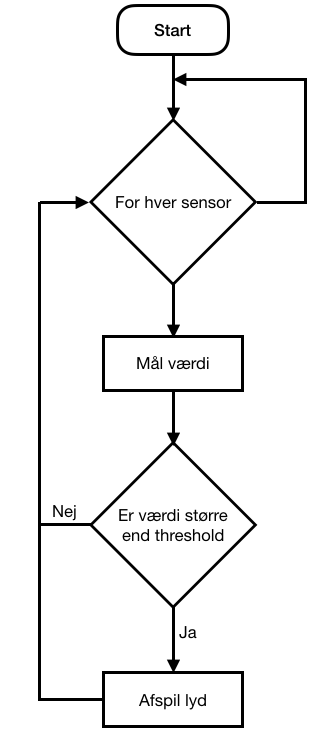
\includegraphics[scale=0.4]{Figure/protoFlowChart01.png}
\caption{
Flowchart for funktionen Afspil lyd. }
\label{fig:protoFlowChart01.png}
\end{figure}

 Programmet baseret på Arduino (https://www.arduino.cc) og Processing (https://processing.org). Kommunikation mellem Arduino og Processing foregår via protokollen Firmata. 
 Arduinoen bruges til at aflæse sensorværdier. De målte værdier sendes, via Firmata, videre til processing som derefter bearbejder informationen.
 Ved at benytte processing kan PC'ens hard
 
 Denne opsætning er valgt for hurtigt og let at konstruerer en fungerende prototype. Via processing kan PC'ens interne hardware tilgås. Derved kan   

\section{1. iteration}
I første iteration 
 Formålet er

processing

\section{2. iteration}
arduino+processing 